% vim:autoindent:set textwidth=78:

\section{Diseñador de impresión}\label{label_printcomposer}

% when the revision of a section has been finalized, 
% comment out the following line:
% \updatedisclaimer

El diseñador de impresión provee crecientes capacidades de diseño e impresión. Permite agregar elementos tales como el map canvas de QGIS, 
leyenda, barra de escala, imágenes, y etiquetas de texto. Puede ajustar tamaño, agrupar, alinear y posicionar cada elemento y ajustar sus propiedades para crear su diseño. El diseño puede ser impreso (también a Postscript y PDF), exportado a formatos de imagen, o a SVG \footnote{Exportar a SVG es soportado, pero no está trabajando apropiadamente con algunas versiones recientes de QT4. Debería intentar y verificar individualmente en su sistema} y puede almacenar el diseño como una plantilla y cargarla nuevamente en otra sesión. Vea una lista de herramientas en la tabla~\ref{tab:printcomposer_tools}:

\begin{table}[h]\index{Print composer!tools}
\centering
\caption{Herramientas del diseñador de impresión}\label{tab:printcomposer_tools}\medskip
 \begin{tabular}{|l|p{6.9cm}|l|p{6.9cm}|}
 \hline \textbf{Ícono} & \textbf{Propósito} & \textbf{Ícono} &
 \textbf{Propósito} \\
 \hline 
\includegraphics[width=0.7cm]{mActionFolder}
 & Cargar desde plantilla &
 
\includegraphics[width=0.7cm]{mActionFileSaveAs} & Guardar como plantilla \\
 \hline 
\includegraphics[width=0.7cm]{mActionExportMapServer}
 & Exportar a un formato imagen & 
 
\includegraphics[width=0.7cm]{mActionSaveAsSVG} & Exportar diseño de impresión 
 a SVG \\
 \hline 
\includegraphics[width=0.7cm]{mActionFilePrint} & Imprimir o 
 exportar como PDF o Postscript &
 
\includegraphics[width=0.7cm]{mActionZoomFullExtent} & Zoom a
 la extensión completa \\
 \hline 
\includegraphics[width=0.7cm]{mActionZoomIn} & Acercar &
 
\includegraphics[width=0.7cm]{mActionZoomOut} & Alejar \\
 \hline 
\includegraphics[width=0.7cm]{mActionDraw} & Refrescar 
 vista &
 
\includegraphics[width=0.7cm]{mActionAddRasterLayer} & Agregar 
 nuevo mapa desde el canvas de mapa de QGIS  \\
 \hline 
\includegraphics[width=0.7cm]{mActionSaveMapAsImage} & Agregar imágenes a  
 diseño de impresión &
 
\includegraphics[width=0.7cm]{mActionLabel} & Agregar etiqueta a diseño de impresión \\
 \hline 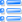
\includegraphics[width=0.7cm]{mActionAddLegend} & Agregar nueva leyenda a 
 diseño de impresión & 
 
\includegraphics[width=0.7cm]{mActionScaleBar} & Agregar nueva barra de escala al diseño de impresión \\
 \hline 
\includegraphics[width=0.7cm]{mActionSelectPan} & Seleccionar/Mover elemento en 
 diseño de impresión &
 
\includegraphics[width=0.7cm]{mActionMoveItemContent} & Mover contenido dentro
 de un elemento \\
 \hline 
\includegraphics[width=0.7cm]{mActionGroupItems} & Agrupar elementos de diseño 
 de impresión & 
 
\includegraphics[width=0.7cm]{mActionUngroupItems} & Desagrupar elementos de diseño 
 de impresión \\
 \hline 
\includegraphics[width=0.7cm]{mActionRaiseItems} & Elevar elementos
 seleccionados  &
 
\includegraphics[width=0.7cm]{mActionLowerItems} & Bajar elementos seleccionados \\
 \hline 
\includegraphics[width=0.7cm]{mActionMoveItemsToTop} & Mover elementos
 seleccionados al frente & 
 
\includegraphics[width=0.7cm]{mActionMoveItemsToBottom} & Mover elementos
 seleccionados al fondo \\
 \hline 
\includegraphics[width=0.7cm]{mActionAlignLeft} & Alinear elementos 
 seleccionados a la izquierda &
 
\includegraphics[width=0.7cm]{mActionAlignRight} & Alinear elementos seleccionados 
 a la derecha \\
 \hline 
\includegraphics[width=0.7cm]{mActionAlignHCenter} & Alinear elementos 
 seleccionados al centro &
 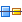
\includegraphics[width=0.7cm]{mActionAlignVCenter} & Alinear elementos seleccionados
 al centro vertical \\
 \hline 
\includegraphics[width=0.7cm]{mActionAlignTop} & Alinear elementos
 seleccionados a arriba &
 
\includegraphics[width=0.7cm]{mActionAlignBottom} & Alinear elementos
 seleccionados a abajo \\
\hline
\end{tabular}
\end{table}

Para acceder al diseñador de impresión, haga clic en el botón \toolbtntwo{mActionFilePrint}{Imprimir}
en la barra de herramientas elija \mainmenuopt{Archivo} > \dropmenuopttwo{mActionFilePrint}{Diseñador de impresión}.

\subsection{Usando el Diseñador de Impresión}\label{label_useprintcomposer} 

Antes que inicie a trabajar con el diseñador de impresión, necesita cargar algunas 
capas raster y vectoriales en el canvas de mapa de QGIS y adaptar sus propiedades 
para ajustarlas a su conveniencia. Después que todo es presentado y simbolizado a 
a su gusto haga clic en el ícono \toolbtntwo{mActionFilePrint}{Diseñador de impresión}.

\begin{figure}[ht]
   \begin{center}
   \caption{Diseñador de Impresión \nixcaption}\label{fig:print_composer_blank}\smallskip
   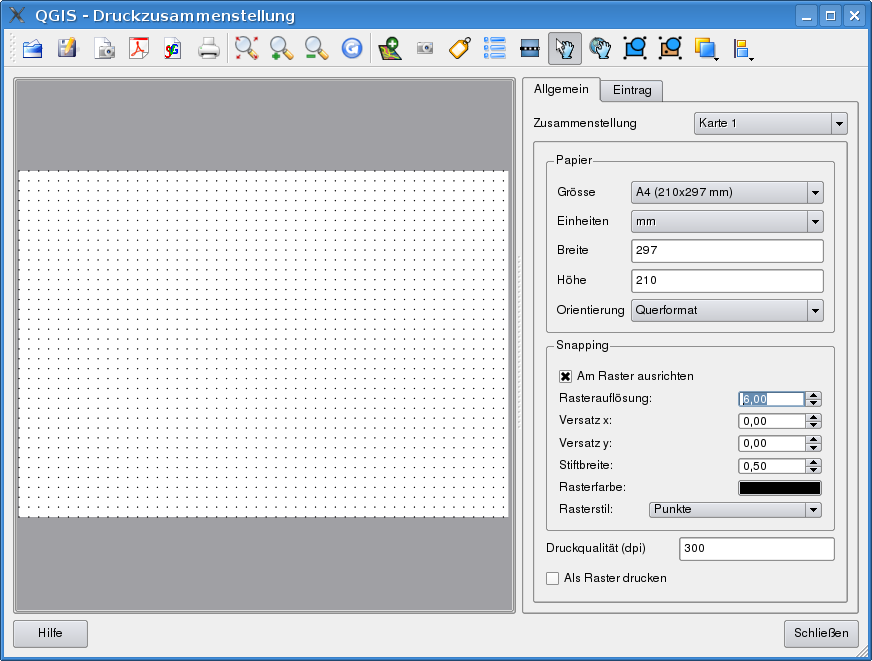
\includegraphics[clip=true, width=\textwidth]{print_composer_blank}
\end{center}  
\end{figure}

Al abrir el diseñador de impresión este le provee un canvas en blanco al cual le puede
agregar el canvas de mapa de QGIS actual, leyenda, barra de escala, imágenes y texto. La figura
\ref{fig:print_composer_blank} muestra la vista inicial del diseñador de impresión 
con un modo activado de \checkbox{Autoensamblado al grid} pero antes de que cualquier elemento haya
sido agregado. El diseñador de impresión provee dos pestañas:

\begin{itemize}
\item La pestaña \tab{General} le permite establecer el tamaño de papel, orientación, la
calidad de impresión para el archivo de salida en dpi y para activar el autoensamblado al grid
de una resolución definida. Note por favor, que la característica \checkbox{Autoensamblar a grid}
solo trabaja, si define una resolución de grid > 0. Además también puede
activar la caja de verificación \checkbox{Imprimir como raster}. Esto significa que todos los elementos
serán rasterizados antes de imprimir o guardar como Postscript o PDF.
\item La pestaña \tab{elemento} muestra las propiedades para el elemento de mapa seleccionado. 
Haga clic el ícono \toolbtntwo{mActionSelectPan}{Seleccionar/Mover elemento} 
para seleccionar un elemento (ej. leyenda, barra de escala o etiqueta) en el canvas. 
Entonces haga clic en la pestaña elemento y personalice las configuraciones para el elemento seleccionado.
\end{itemize}

Puede agregar múltiples elementos al diseñador. También es posible tener 
mas de una vista del mapa, leyenda o barra de escala en al canvas del diseñador de impresión. 
Cada elemento tiene sus propias propiedades y en el caso del mapa, su propia 
extensión.

\subsubsection{Añadir el canvas del mapas actual de QGIS al diseñador de impresión}

Para añadir el canvas de Qgis al mapa, haga clic en el botón \toolbtntwo{mActionAddRasterLayer}{Añadir nuevo mapa desde el canvas de Qgis} en la barra del diseñador de impresión y arrastre un 
rectángulo en el canvas del diseñador con el botón izquierdo del ratón para agregarlo al mapa. 
Usted verá una caja vacía con un mensaje \textit{"El mapa será impreso aquí"}.
Para mostrar el mapa actual, puede elegir entre tres modos diferentes en el mapas en la pestaña \tab{Elemento}:

\begin{itemize}
\item \selectstring{Vista previa}{Rectángulo} es la configuración predeterminada. Solo muestra
una caja vacía con un mensaje \textit{"El mapa será impreso aquí"}. 
\item \selectstring{Vista previa}{Cache} muestra el mapa en la resolución actual de la ventana. En caso que se acerque o aleje en la ventana del diseñador, el mapas no es visualizado nuevamente
pero la imagen será escalada.
\item \selectstring{Vista previa}{Representar} significa, que si acerca o aleja la 
ventana del diseñador, el mapa será representado nuevamente, pero por razones de espacio, solo
hasta una resolución máxima.
\end{itemize}

\begin{figure}[ht]
\centering
\caption{Diseñador de impresión, contenido de mapa de la pestaña elemento \nixcaption}\label{fig:print_composer_map_item}
   \subfigure[Ancho , alto y diálogo de extensión] {\label{subfig:print_composer_map_item1}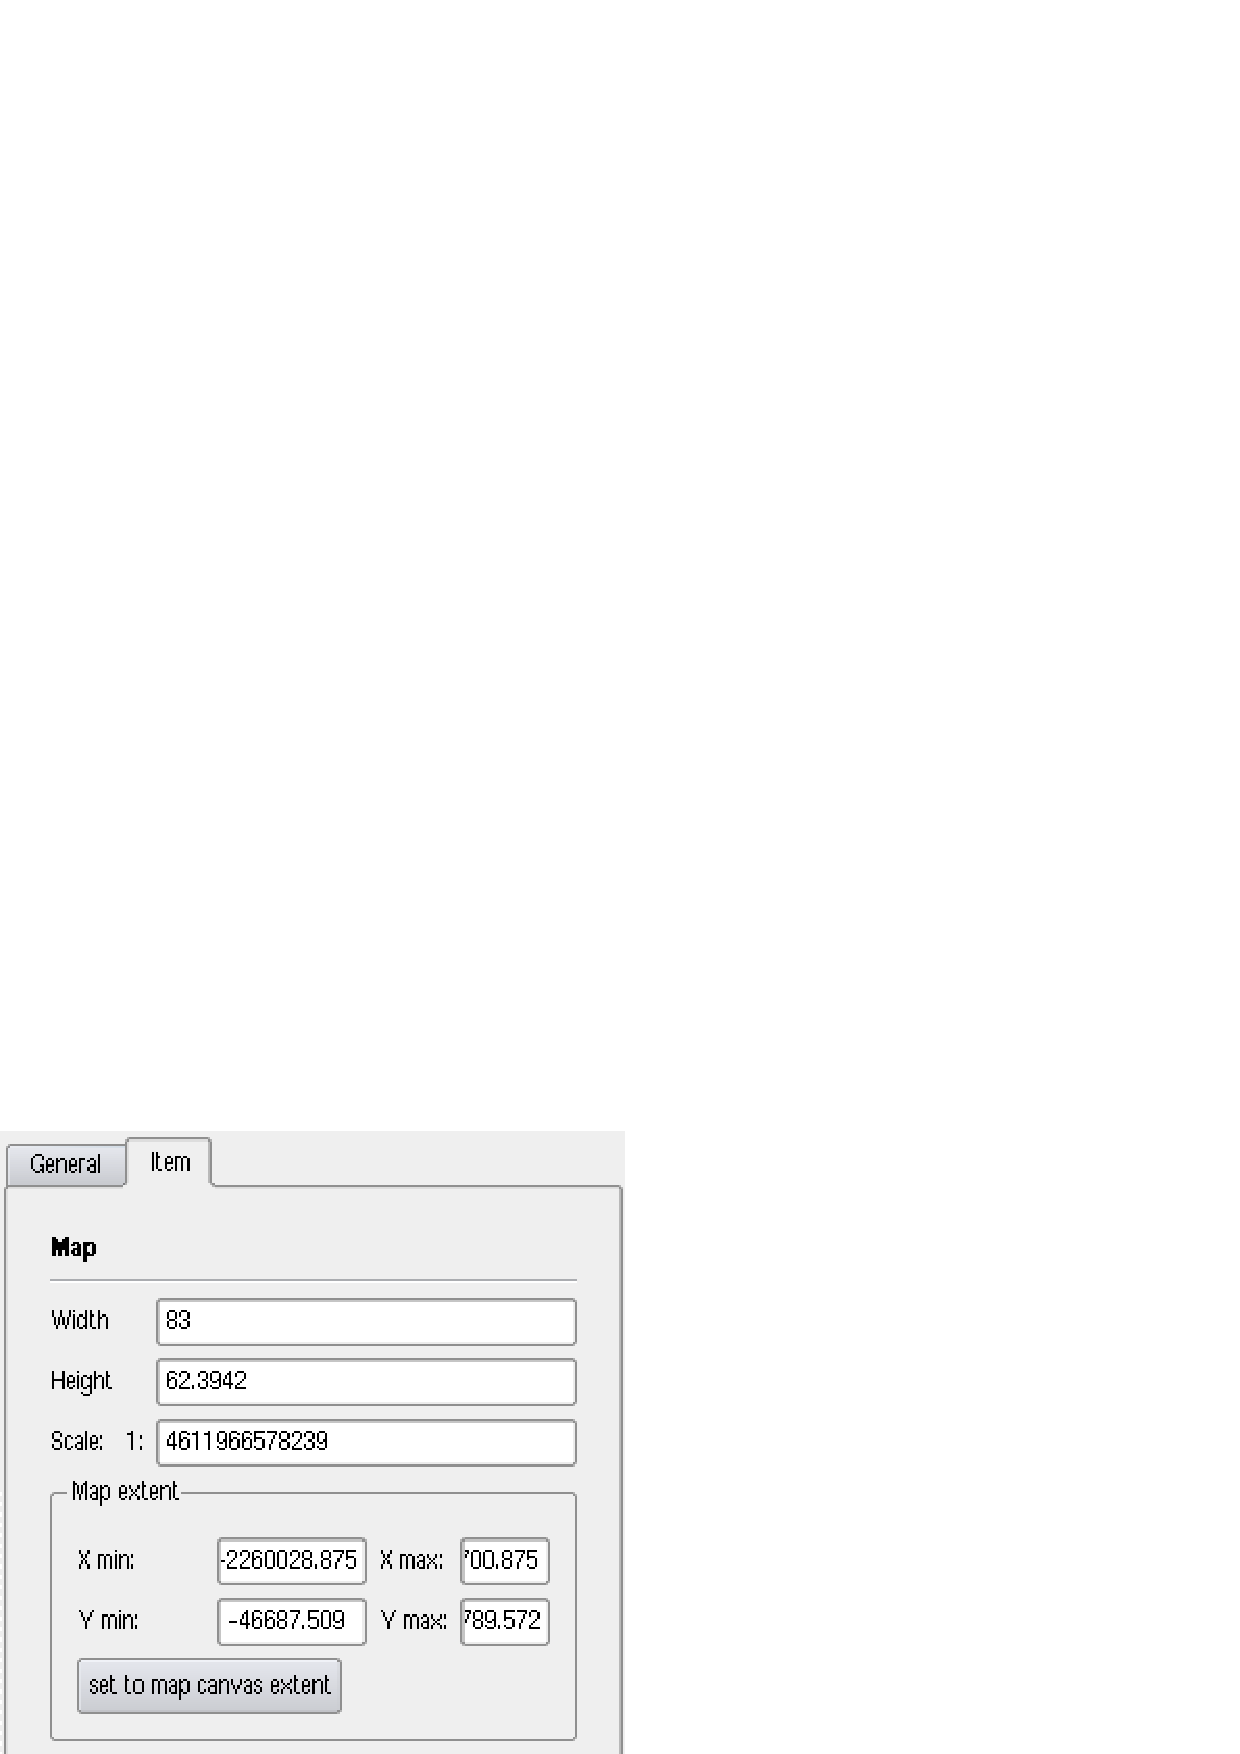
\includegraphics[clip=true, width=0.4\textwidth]{print_composer_map_item1}}\goodgap
   \subfigure[Properties dialog] {\label{subfig:print_composer_map_item2}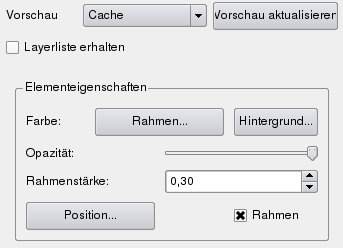
\includegraphics[clip=true, width=0.4\textwidth]{print_composer_map_item2}}
\end{figure}

Puede cambiar el tamaño del mapa haciendo clic en el botón \toolbtntwo{mActionSelectPan}{Seleccionar/Mover elemento}, seleccionando el elemento, y arrastrando una de las asas azules en las esquinas del mapa. Con el mapa seleccionado, ahora puede adaptar mas propiedades en mapa de la pestaña \tab{Elemento}. Cambiar el tamaño del elemento mapa especificando el ancho, altura o escala. Definir la extensión del mapa usando valores Y y 
X min/max o haciendo clic en el botón \button{establecer extensión del canvas del mapas}. Actualizar la 
vista previa del mapa y seleccionar, entre ver desde cache o un rectángulo  con un mensaje 
\textit{" El mapa será impreso aquí"}. Definir colores ancho del contorno para el elemento 
marco, establecer un color de fondo y opacidad para el canvas del mapa. También puede seleccionar 
o deseleccionar para mostrar un elemento marco con la caja de selección \checkbox{marco}  
(vea la figura ~\ref{fig:print_composer_map_item}). Si cambia la vista en el canvas del mapa de QGIS 
haciendo zoom, moviendose o cambiando las propiedades de vectores o raster, puede actualizar  
el diseñador de impresión seleccionando el elemento mapa y haciendo clic 
en el botón \button{Actualizar vista previa} en el elemento mapa de la pestaña \tab{Elemento} 
(vea la figura~\ref{fig:print_composer_map_item}). 

Para mover capas dentro del elemento mapa seleccione el elemento mapa, haciendo clic 
en el ícono \toolbtntwo{mActionMoveItemContent}{Mover contenido del elemento} 
y mueva las capas dentro del elemento frame del mapa con el botón izquierdo del ratón.

\subsubsection{Herramientas de navegación}

Para la navegación en el mapa el diseñador de impresión provee 4 herramientas generales:

\begin{itemize}
\item \toolbtntwo{mActionZoomOut}{Acercar},
\item \toolbtntwo{mActionZoomOut}{Alejar},
\item \toolbtntwo{mActionZoomFullExtent}{Zoom a extensión completa} y
\item \toolbtntwo{mActionDraw}{Refrescar la vista}, si encuentra la vista en un estado inconsistente.
\end{itemize}


\subsubsection{Añadir otros elementos al diseñador de impresión} 

Además de agregar el canvas del mapa actual al diseñador de impresión, también es posible 
agregar, posicionar, mover y personalizar leyenda, barra de escala, imágenes y etiquetas.

\minisec{Etiquetas e imágenes}

Para agregar etiquetas a una imagen, haga clic en el ícono \toolbtntwo{mActionLabel}{Añadir etiqueta} o 
\toolbtntwo{mActionSaveMapAsImage}{Añadir imagen}, colocar un elemento con
el botón en el canvas del diseñador de impresión, posicionar y personalizar
su apariencia en la pestaña \tab{Elemento}. 

\begin{figure}[ht]
\centering
\caption{Personalizar etiquetas e imágenes del diseñador de impresión \nixcaption}\label{fig:print_composer_tab2}
   \subfigure[etiqueta pestaña elemento] {\label{subfig:print_composer_label_item}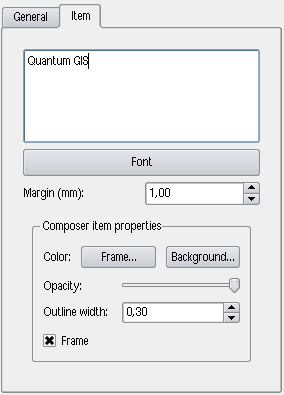
\includegraphics[clip=true, width=0.4\textwidth]{print_composer_label_item}}\goodgap
   \subfigure[imagen pestaña elemento] {\label{subfig:print_composer_image_item}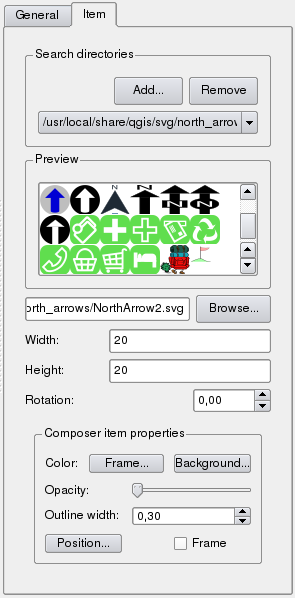
\includegraphics[clip=true, width=0.4\textwidth]{print_composer_image_item}}
\end{figure}

\minisec{Leyenda y barra de escala}

Para añadir una leyenda de mapa o una barra de escala, haga clic en \toolbtntwo{mActionAddLegend}{Añadir nueva leyenda} o 
\toolbtntwo{mActionScaleBar}{Añadir nueva barra de escala}, colocar el elemento con el botón izquierdo del ratón en el canvas del diseñador de impresión, posicionar y personalizar su apariencia en la pestaña \tab{Elemento}.

\begin{figure}[ht]
\centering
\caption{Personalizar la leyenda y barra de escala del diseñador de impresión \nixcaption}\label{fig:print_composer_tab1}
   \subfigure[leyenda pestaña elemento] {\label{subfig:print_composer_legend_item}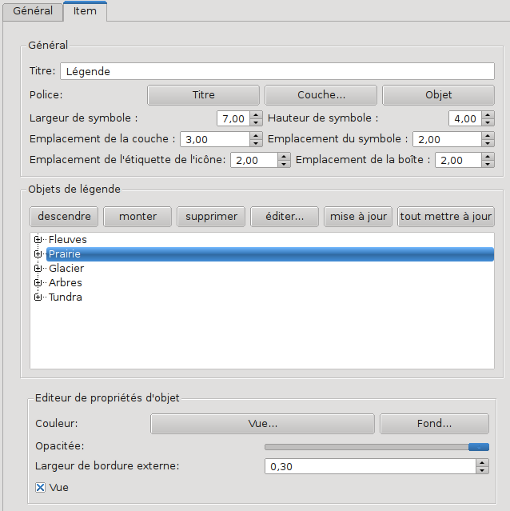
\includegraphics[clip=true, width=0.4\textwidth]{print_composer_legend_item}}\goodgap
   \subfigure[barra de escala pestaña elemento] {\label{subfig:print_composer_scalebar_item}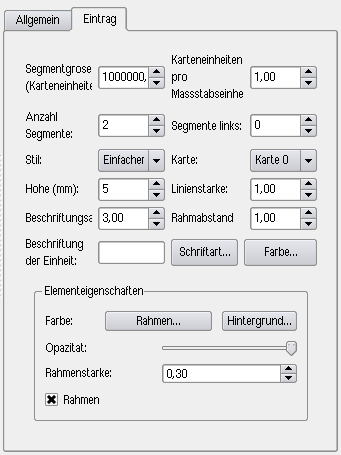
\includegraphics[clip=true, width=0.4\textwidth]{print_composer_scalebar_item}}
\end{figure}

\subsubsection{Levantar, bajar y alinear elementos}

Las funcionalidades de levantar y bajar elementos están dentro del menú desplegable 
\toolbtntwo{mActionRaiseItems}{Levantar elementos seleccionados}. Elija un elemento
del canvas del diseñador de impresión y seleccione la funcionalidad coincidente a
levantar o bajar el elemento seleccionado comparado a los otros elementos (vea la
tabla~\ref{tab:printcomposer_tools}). 

Hay múltiples funcionalidades de alineación disponibles dentro del menú desplegable
\toolbtntwo{mActionAlignLeft}{Alinear elementos seleccionados} (vea la
tabla~\ref{tab:printcomposer_tools}). Para usar la funcionalidad de alineación , primero
seleccione algunos elementos y entonces haga clic en el ícono de alineación que coincida. Todo
lo seleccionado será entonces alineado dentro de un cuadro delimitador común.       

\subsubsection{Creando la salida}

La figura \ref{fig:print_composer_complete} muestra la salida del diseñador de impresión con un ejemplo 
de diseño de impresión incluyendo cada tipo de elemento de mapa descrito en las secciones de arriba.

\begin{figure}[h]
   \begin{center}
   \caption{Diseñador de impresión con vista de mapa, leyenda, barra de escala, y texto agregados \nixcaption}
   \label{fig:print_composer_complete}\smallskip
   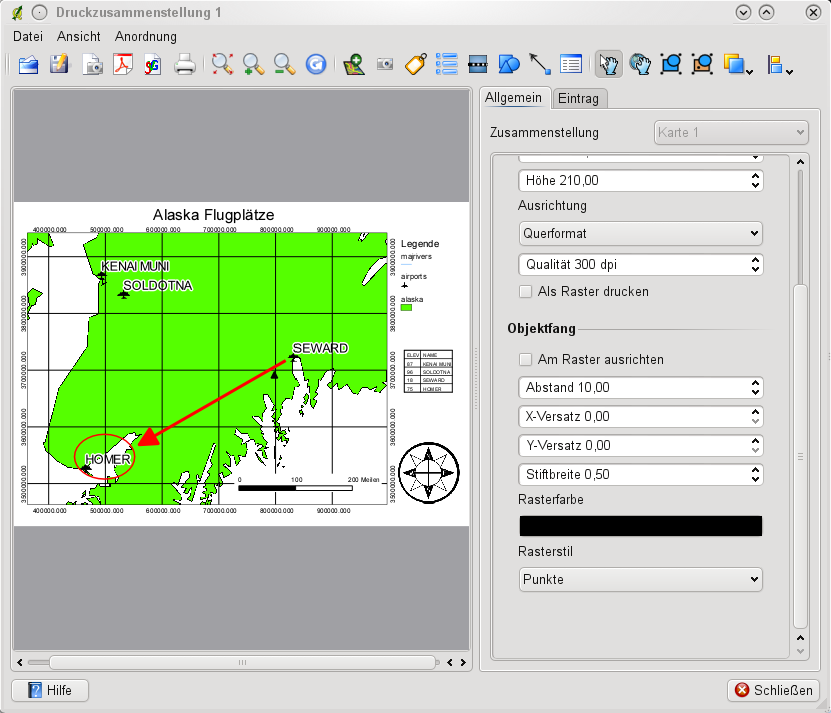
\includegraphics[clip=true, width=\textwidth]{print_composer_complete}
\end{center}  
\end{figure}

El diseñador de impresión le permite crear múltiples formatos de salida y es posible definir 
la resolución (calidad de impresión) y tamaño de papel:

\begin{itemize}
\item El ícono \toolbtntwo{mActionFilePrint}{Imprimir} permite imprimir el diseño 
a una impresora conectada o como archivo PDF o Postscript dependiendo de los controladores 
de impresora instalados.
\item El ícono \toolbtntwo{mActionExportMapServer}{Exportar como imagen} exporta el 
canvas del diseñador en múltiples formatos de imágenes como PNG, BPM, TIF, JPG, \dots
\item El ícono \toolbtntwo{mActionSaveAsSVG}{Exportar como SVG} guarda el canvas del diseñador 
de impresión como un SVG (Gráficas Vectoriales Escalables). \textbf{Nota:} Actualmente la 
salida SVG es muy básica. Este no es un problema de QGIS, sino un problema de la  
librería Qt. Esto esperamos sea corregido en futuras versiones.
\end{itemize}

\subsubsection{Guardando y cargando una plantilla del diseñador de impresión}

Con los íconos \toolbtntwo{mActionFileSaveAs}{Guardar como plantilla} y
\toolbtntwo{mActionFolder}{Cargar como plantilla} puede guardar el estado actual
de la sesión del diseñador de impresión como una  plantilla *.qpt y cargar la plantilla
nuevamente en otra sesión.

